\section{Previous Work}
The existing implementation of the \gls{sdr} workflow for high energy
accelerator-driven nuclear systems determine the nuclear inventory changes at
the resolution of a geometric cell. This workflow uses a specialized tally
during the first transport step to collect the nuclear inventory changes. This
workflow can be seen in Figure \ref{fig:cell_rnucs}.
\begin{figure}[H]
        \centering
        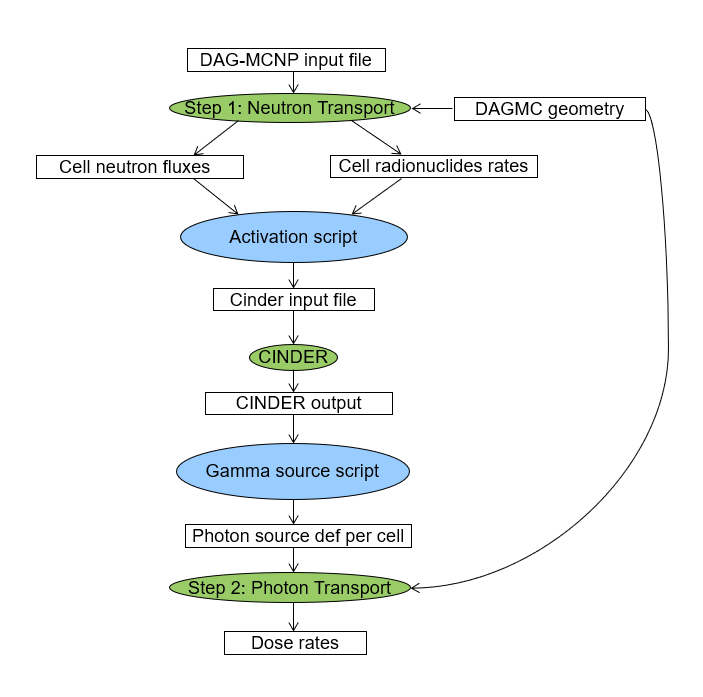
\includegraphics[scale=0.4]{../figs/rnucs_r2s.png}
        \caption{Cell based \gls{sdr}-rnucs Workflow}
        \label{fig:cell_rnucs}
\end{figure}
This workflow requires a patch to modify the \gls{mcnp} source code to add
\gls{dag} and the specialized tally \emph{rnucs}. The \emph{rnucs} tally
collects nuclide production and destruction rates. The workflow is then
automated with a perl script to collect information flux and nuclide
information, write input files and run an activation calculation per geometric
cell of interest. Another script is then used to write an \gls{mcnp}
\emph{sdef} card to use in the photon transport.
\newpage
